\section{Preliminary}

\subsection{Proximal Policy Optimization (PPO)}
PPO~\cite{schulman2017proximal} introduces a clipped surrogate objective for policy optimization. By constraining the policy updates within a proximal region of the previous policy using clip, PPO stabilizes training and improves sample efficiency. Specifically, PPO updates the policy by maximizing the following objective:
\begin{equation}
\begin{aligned}
\mathcal{J}_\text{PPO}(\theta) = \mathbb{E}_{(q,a)\sim \mathcal{D},o_{\le t}\sim\pi_{\theta_{\text{old}}}(\cdot\mid q)}
\Bigg[ 
\min \Bigg( \frac{\pi_{\theta}(o_t\mid q,o_{<t})}{\pi_{\theta_{\text{old}}}(o_t\mid q,o_{<t})} \hat{A}_t,  
\ \text{clip} \Bigg( \frac{\pi_{\theta}(o_t\mid q,o_{<t})}{\pi_{\theta_{\text{old}}}(o_t\mid q,o_{<t})}, 1 - \varepsilon, 1 + \varepsilon \Bigg) \hat{A}_t \Bigg) \Bigg],
\label{eq:ppoloss}
\end{aligned}
\end{equation}
where $(q,a)$ is a question-answer pair from the data distribution $\mathcal{D}$, $\varepsilon$ is the clipping range of importance sampling ratio, and $\hat{A}_t$ is an estimator of the advantage at time step $t$. Given the value function $V$ and the reward function $R$, $\hat{A}_t$ is computed using the Generalized Advantage Estimation (GAE)~\cite{schulman2018highdimensionalcontinuouscontrolusing}:
\begin{equation}
\begin{aligned}
    &\hat{A}_t^{\text{GAE}(\gamma,\lambda)} = \sum_{l=0}^{\infty}(\gamma\lambda)^l\delta_{t+l},
\end{aligned}
\end{equation}
where
\begin{equation}
    \delta_{l}=R_l+\gamma V(s_{l+1})-V(s_l),\quad 0\le\gamma,\lambda\le1.
\end{equation}


\subsection{Group Relative Policy Optimization (GRPO)}

Compared to PPO, GRPO eliminates the value function and estimates the advantage in a group-relative manner. For a specific question-answer pair $(q,a)$, the behavior policy $\pi_{\theta_\text{old}}$ samples a group of $G$ individual responses $\{ o_i\}_{i=1}^G$. Then, the advantage of the $i$-th response is calculated by normalizing the group-level rewards $\{ R_i \}_{i=1}^G$:
\begin{equation}
\hat{A}_{i,t} = \frac{r_i - \text{mean}(\{R_i\}_{i=1}^G)}{\text{std}(\{R_i\}_{i=1}^G)}.
\end{equation}

Similar to PPO, GRPO adopts a clipped objective, together with a directly imposed KL penalty term:
% Additionally, the KL-regularization between current policy $\pi_\theta$ and the reference policy $\pi_\text{ref}$ is directly added to the loss function:
\begin{equation}
\begin{aligned}
\mathcal{J}_\text{GRPO}(\theta)& = \mathbb{E}_{(q,a)\sim \mathcal{D}, \{o_i\}_{i=1}^G\sim \pi_{\theta_\text{old}}(\cdot\mid q)} \\&
\Bigg[ \frac{1}{G}\sum_{i=1}^{G} \frac{1}{|o_i|}\sum_{t=1}^{|o_i|} \Bigg( 
\min \Big( r_{i,t}(\theta) \hat{A}_{i,t},  
\ \text{clip} \Big( r_{i,t}(\theta), 1 - \varepsilon, 1 + \varepsilon \Big) \hat{A}_{i,t} \Big)
- \beta D_{\text{KL}}(\pi_{\theta} || \pi_{\text{ref}}) 
\Bigg) \Bigg],
\label{eq:grpoloss}
\end{aligned}
\end{equation}
where
\begin{equation}
    r_{i,t}(\theta)=\frac{\pi_{\theta}(o_{i,t} \mid q, o_{i,<t})}{\pi_{\theta_{\text{old}}}(o_{i,t} \mid q,o_{i,<t})}.
\end{equation}

It is also worth noting that GRPO computes the objective at the sample-level. To be exact, GRPO first calculates the mean loss within each generated sequence, before averaging the loss of different samples. As we will be discussing in Section~\ref{sec:tokenlevel}, such difference may have an impact on the performance of the algorithm.


\begin{figure}[t]
    \centering
    \begin{subfigure}{0.49\textwidth}
        \centering
        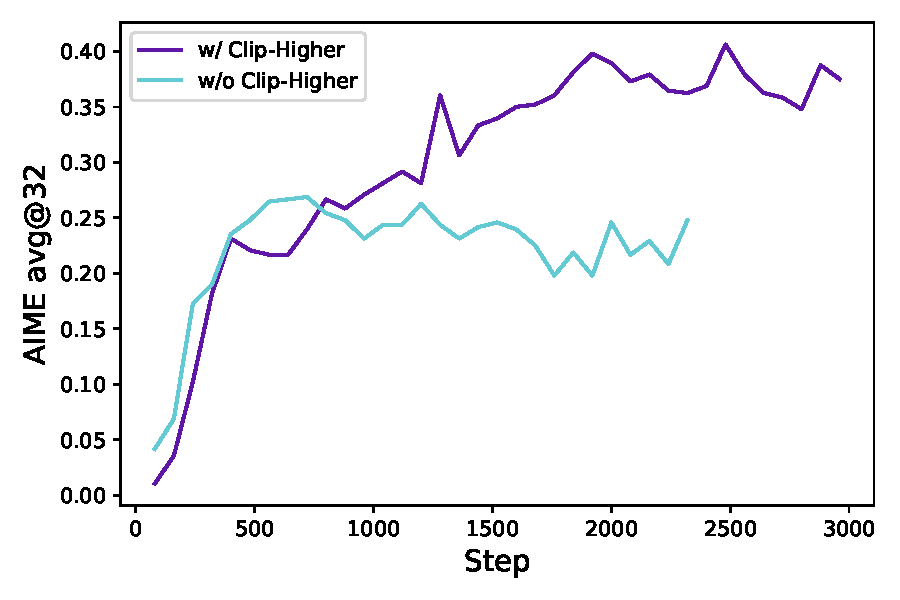
\includegraphics[width=\textwidth]{figures/3.1.2.pdf}
        \caption{Accuracies on AIME.}
        \label{fig:clighigh_acc}
    \end{subfigure}
    \hfill
    \begin{subfigure}{0.49\textwidth}
        \centering
        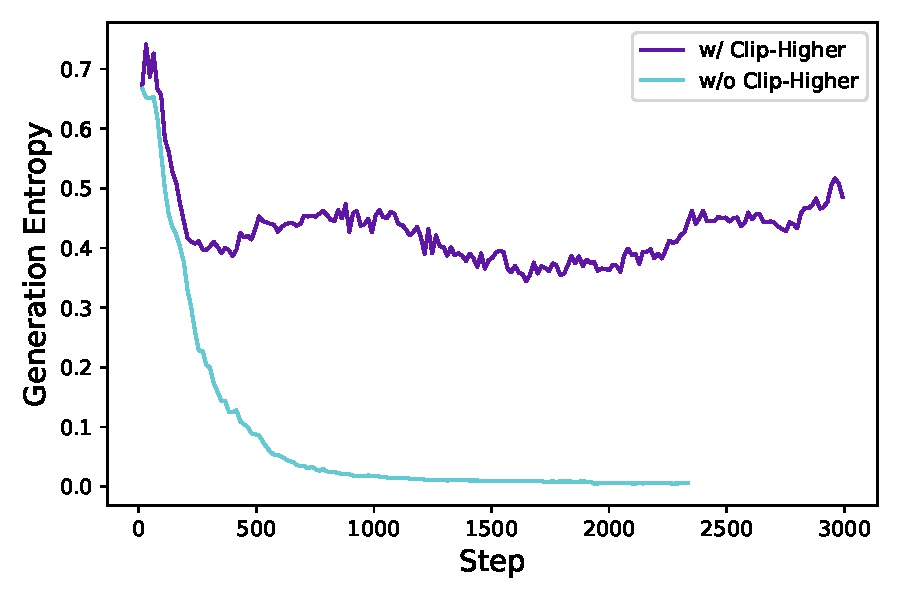
\includegraphics[width=\textwidth]{figures/3.1.1.pdf}
        \caption{Entropy of actor model.}
        \label{fig:cliphigh_entropy}
    \end{subfigure}
    \caption{The accuracy on the AIME test set and the entropy of the actor model's generated probabilities during the RL training process, both before and after applying \textbf{Clip-Higher} strategy.}
    \label{fig:clip_high}
\end{figure}


\subsection{Removing KL Divergence}
\label{sec:removekl}
The KL penalty term is used to regulate the
divergence between the online policy and the frozen reference policy. 
In the RLHF scenario~\cite{NEURIPS2022_b1efde53}, the goal of RL is to align the model behavior without diverging too far from the initial model.
However, during training the long-CoT reasoning model, the model distribution can diverge significantly from the initial model, thus this restriction is not necessary. Therefore, we will exclude the KL term from our proposed algorithm.

\subsection{Rule-based Reward Modeling}
The use of reward model usually suffers from the reward hacking problem~\cite{amodei2016concreteproblemsaisafety,
everitt2017reinforcementlearningcorruptedreward,
google2020specialgaming,
everitt2021rewardtamperingproblemssolutions,
gao2022scalinglawsrewardmodel,weng2024rewardhack}.
Instead, we directly use the final accuracy of a verifiable task as the outcome reward, computed using the following rule:
\begin{equation}
    R(\hat{y}, y) = 
    \begin{cases} 
    1, & \texttt{is\_equivalent}(\hat{y}, y) \\
    -1, & \text{otherwise} 
    \end{cases}
\end{equation}
where $y$ is the ground-truth answer and $\hat{y}$ is the predicted answer.
This is proved to be an effective approach to activating the base model's reasoning capability, as shown in multiple domains such as automated theorem proving~\cite{polu2020generativelanguagemodelingautomated,trinh2024solving,google2024alphageometry,google2024alphaproofandalphageometry}, computer programming~\cite{le2022coderl,shinn2023reflexionlanguageagentsverbal,chen2023teachinglargelanguagemodels,gehring2025rlefgroundingcodellms}, and mathematics competition~\cite{guo2025deepseek}.

